\documentclass[11pt]{report}
% this template is originally from Roy Dong's ECE 515.
% Edited by Dawei Sun
%%%%%%%%%%%%%%%%%%%%%%%%%%%%%%%%%%%%%%%%%%%%%%%%%%%%%%%%%%%%%%%%%%
% Set the margins of our document.
\usepackage[margin = 1 in]{geometry}

%%%%%%%%%%%%%%%%%%%%%%%%%%%%%%%%%%%%%%%%%%%%%%%%%%%%%%%%%%%%%%%%%%
% Import commands for custom header.
\usepackage{fancyhdr}
\pagestyle{fancy}

%%%%%%%%%%%%%%%%%%%%%%%%%%%%%%%%%%%%%%%%%%%%%%%%%%%%%%%%%%%%%%%%%%
% Allow ourselves to do equations!
\usepackage{amsmath,amssymb,amsthm,amsfonts}
\usepackage{upgreek}
\usepackage{mathtools}

%%%%%%%%%%%%%%%%%%%%%%%%%%%%%%%%%%%%%%%%%%%%%%%%%%%%%%%%%%%%%%%%%%
% Nicer formatting for enumerate commands.
\usepackage[shortlabels]{enumitem}

\usepackage{algorithm2e}
\usepackage[noend]{algpseudocode}

%%%%%%%%%%%%%%%%%%%%%%%%%%%%%%%%%%%%%%%%%%%%%%%%%%%%%%%%%%%%%%%%%%
% Colored text and include images.
\usepackage{color}
\usepackage{graphicx}

\usepackage{listings}
\usepackage{multicol}
%%%%%%%%%%%%%%%%%%%%%%%%%%%%%%%%%%%%%%%%%%%%%%%%%%%%%%%%%%%%%%%%%%
% Some custom macros to make life easier.
\newcommand{\mc}{\mathcal}
\newcommand{\mb}{\mathbb}

\newcommand{\T}{\intercal}
\newcommand{\E}[1]{\mathbb{E}\left[#1\right]}

%%%%%%%%%%%%%%%%%%%%%%%%%%%%%%%%%%%%%%%%%%%%%%%%%%%%%%%%%%%%%%%%%%
%%%%%%%%%%%%%%%%%%%%%%%%%%%%%%%%%%%%%%%%%%%%%%%%%%%%%%%%%%%%%%%%%%
%%%%%%%%%%%%%%%%%%%%%%%%%%%%%%%%%%%%%%%%%%%%%%%%%%%%%%%%%%%%%%%%%%

\lhead{ECE 553 - Fall 2020 at University of Illinois at Urbana-Champaign}
\rhead{\textcolor{red}{Dawei Sun (daweis2)}}

%%%%%%%%%%%%%%%%%%%%%%%%%%%%%%%%%%%%%%%%%%%%%%%%%%%%%%%%%%%%%%%%%%
%%%%%%%%%%%%%%%%%%%%%%%%%%%%%%%%%%%%%%%%%%%%%%%%%%%%%%%%%%%%%%%%%%
%%%%%%%%%%%%%%%%%%%%%%%%%%%%%%%%%%%%%%%%%%%%%%%%%%%%%%%%%%%%%%%%%%

\begin{document}

%%%%%%%%%%%%%%%%%%%%%%%%%%%%%%%%%%%%%%%%%%%%%%%%%%%%%%%%%%%%%%%%%%
%%%%%%%%%%%%%%%%%%%%%%%%%%%%%%%%%%%%%%%%%%%%%%%%%%%%%%%%%%%%%%%%%%
%%%%%%%%%%%%%%%%%%%%%%%%%%%%%%%%%%%%%%%%%%%%%%%%%%%%%%%%%%%%%%%%%%

\section*{Exercise 1.1}
Not necessary. There are two cases: 1. The set of feasible directions is not compact; 2. The feasible set $D$ is not convex.
\begin{figure}
    \centering
    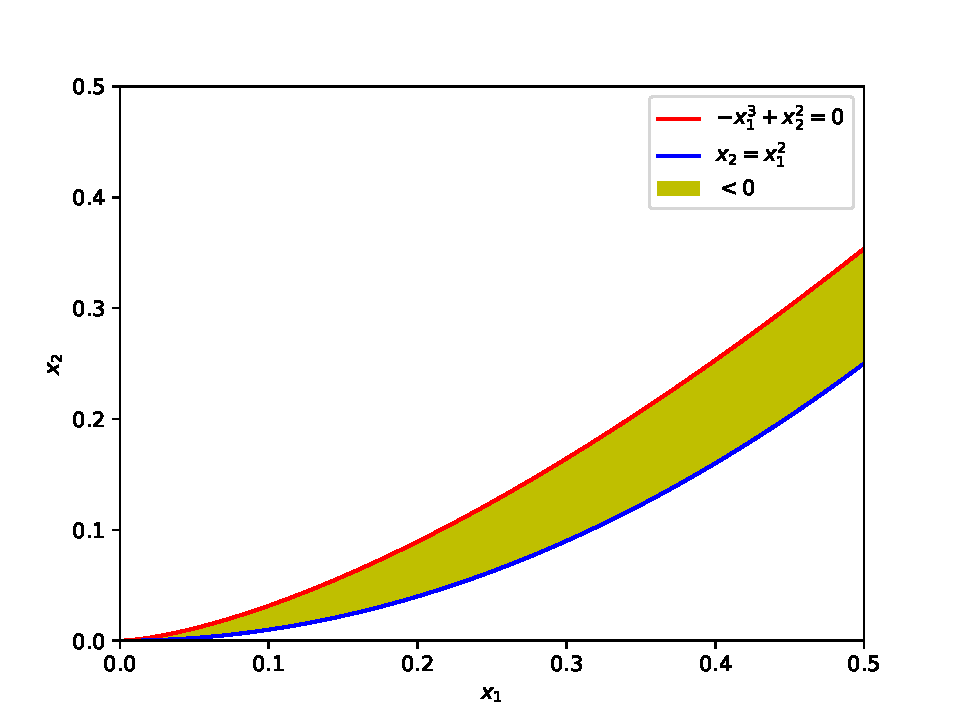
\includegraphics[width=0.45\linewidth]{ECE553/hw1/ece553_hw1_1.pdf}
    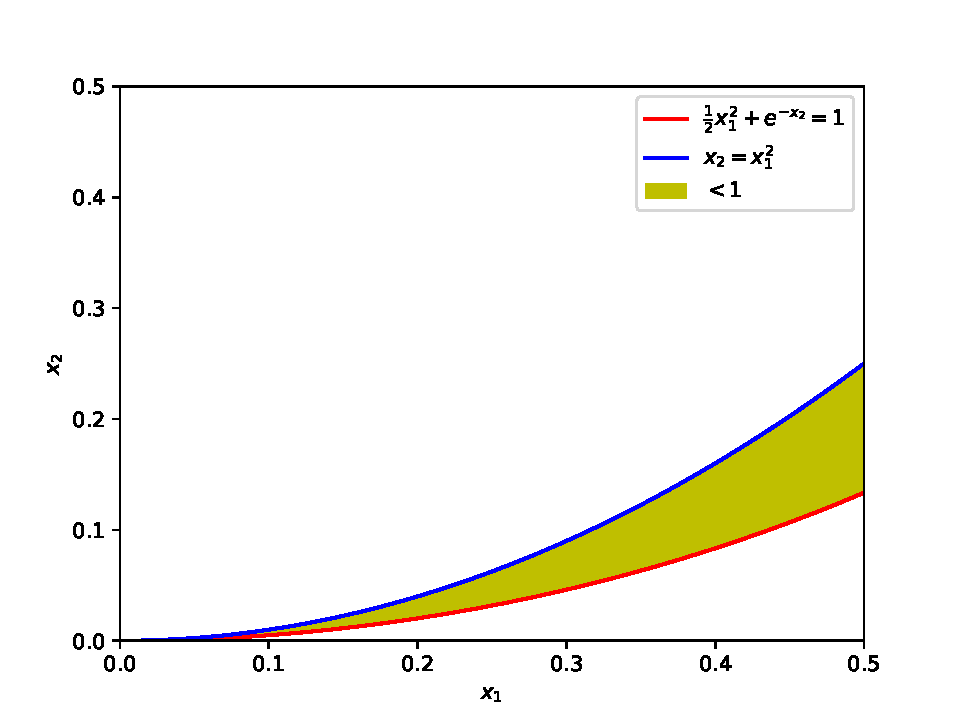
\includegraphics[width=0.45\linewidth]{ECE553/hw1/ece553_hw1_2.pdf}
    \caption{Counterexample 1 and Counterexample 2.}
    \label{fig:fig1}
\end{figure}
\paragraph{Counterexample 1} (The set of feasible directions is not compact.) Let $f(x) = -x_1^3 + x_2^2$ and the feasible set $D = \{x \in \mathbb{R}^2: x_1 \geq 0, x_2 \geq x_1^2\}$. Consider the origin $x* = (0, 0)$. Then, obviously the set of nonzero feasible directions at $x^*$ is $\{d\in\mathbb{R}^2: d_1 \geq 0, d_2 > 0\}$, which is not closed (thus, not compact). We have that $\nabla f(x^*) = [0, 0]$ and $\nabla^2 f = \begin{bmatrix}0 & 0\\0 & 2\end{bmatrix}$. Thus, for all valid $d$, $\nabla f(x^*) \cdot d = 0$ and $d^\T \nabla^2 f(x^*) d = 2 d_2^2 > 0$. However, as shown in Figure~\ref{fig:fig1}, $x^*$ is not a minimum.
% For any $\epsilon \in (0,1)$, considering the point $\hat{x} = (\epsilon / 2, \epsilon^2 / 4)$, we have that $\|\hat{x}\|^2 = \epsilon^2/4 + \epsilon^4/16 \leq \epsilon^2$, and thus $\hat{x}$ is in the $\epsilon$-ball around $x^*$. However, $f(\hat{x}) = -\epsilon^3/8 + \epsilon^4/16 = \epsilon^3(\epsilon/16 - 1/8) < 0 = f(x^*)$, and thus $x^*$ is not a local minimum.
\paragraph{Counterexample 2} (The feasible set is not convex.) Let $f(x) = \frac{1}{2}x_1^2 + e^{-x_2}$ and the feasible set be $D = \{x \in \mathbb{R}^2: x_2 \leq x_1^2\}$. Then, consider the point $x^* = (0,0)$. We have that $\nabla f(x^*) = [0, -1]$ and $\nabla^2 f = \begin{bmatrix}1 & 0\\0 & 1\end{bmatrix}$. Then, obviously the set of nonzero feasible directions at $x^*$ is just $\{d \in \mathbb{R}^2: d_2 \leq 0\}/\{(0,0)\}$. Thus, for all valid $d$, $\nabla f(x^*) \cdot d = -d_2 \geq 0$ and $d^\T \nabla^2 f(x^*) d = d_1^2 + d_2^2 > 0$. However, as shown in Figure~\ref{fig:fig1}, $x^*$ is not a minimum. More formally, considering the points on the boundary such that $x_2 = x_1^2$, then $g(x_2) = f(x) = \frac{1}{2}x_2 + e^{-x_2}$. Since $g'(0) = \frac{1}{2} - 1 < 0$, $g(x_2)$ decreases in $[0,\epsilon)$ for some $\epsilon > 0$, which means there exists some points on the boundary with smaller value than $f(x^*)$.

\section*{Exercise 1.2}
A counterexample is as follows.
\begin{align*}
& \min f(x_1, x_2) = x_2\\
& \text{subject to}\\
& h_1(x_1, x_2) = 3x_1 - x_2^2 = 0\\
& h_2(x_1, x_2) = x_1 - x_2^2 = 0\\
\end{align*}
First, the feasible set contains only one point $D = \{(0,0)\}$, and thus $x^* = (0,0)$ is a minimum. We have that $\nabla f(x^*) = [0,1]$, $\nabla h_1(x^*) = [3, 0]$, and $\nabla h_2(x^*) = [1, 0]$. Thus, $\nabla h_1(x^*)$ and $\nabla h_2(x^*)$ are linearly dependent, and $\nabla f(x^*)$ can not be represented as a linear combination of $\nabla h_1(x^*)$ and $\nabla h_2(x^*)$.

\section*{Exercise 1.3}
Considering the mapping associated with $m+1$ direction vectors $d_1,\cdots,d_{m+1}$, $F(\alpha_1,\cdots,\alpha_{m+1}) = \left(f(x^*+\sum_{i=1}^{m+1}\alpha_i d_i), h_1(x^*+\sum_{i=1}^{m+1}\alpha_i d_i), \cdots, h_{m}(x^*+\sum_{i=1}^{m+1}\alpha_i d_i)\right)$. The Jacobian of $F$ at the origin is
\[\nabla F|_{\alpha = 0} = \begin{bmatrix} \nabla f(x^*) \cdot d_1 & \cdots & \nabla f(x^*) \cdot d_{m+1}\\
~~~~A~~~~~~~~~~~~~~&|&~~~~b
\end{bmatrix},
\] where $A = \begin{bmatrix} \nabla^\T h_1(x^*) & \cdots & \nabla^\T h_{m}(x^*)
\end{bmatrix}^\T \begin{bmatrix} d_1 & \cdots & d_{m}
\end{bmatrix}$ and $b = \begin{bmatrix} \nabla^\T h_1(x^*) & \cdots & \nabla^\T h_{m}(x^*)
\end{bmatrix}^\T d_{m+1}$. Since $x^*$ is a regular point, rows of $\begin{bmatrix} \nabla^\T h_1(x^*) & \cdots & \nabla^\T h_{m}(x^*)
\end{bmatrix}^\T$ are linearly independent. Thus, there must exists $\begin{bmatrix} d_1 & \cdots & d_{m}
\end{bmatrix}$ such that the rows of $A$ are linearly independent. For such a $\begin{bmatrix} d_1 & \cdots & d_{m}
\end{bmatrix}$, there exists a unique linear decomposition $\nabla f(x^*) \begin{bmatrix} d_1 & \cdots & d_{m}\end{bmatrix} = \begin{bmatrix}\lambda_1 & \cdots & \lambda_m\end{bmatrix} A$, since the rows of $A$ are linearly independent. Since $x^*$ is a minimum, we must have that the Jacobian is singular, and thus rows of $\nabla F|_{\alpha = 0}$ are linearly dependent, which implies $\nabla f(x^*) \cdot d_{m+1} = \begin{bmatrix}\lambda_1 & \cdots & \lambda_m\end{bmatrix} b$ for all $d_{m+1}$. Therefore, we must have $\nabla f(x^*) = \begin{bmatrix}\lambda_1 & \cdots & \lambda_m\end{bmatrix} \begin{bmatrix} \nabla^\T h_1(x^*) & \cdots & \nabla^\T h_{m}(x^*)
\end{bmatrix}^\T$.

\section*{Exercise 1.4}
Considering the following optimization problem.
\begin{align*}
&\min f(x) = \|x-y\| + \|x-z\|\\
&\text{subject to}\\
&h(x) = 0
\end{align*}
The first-order necessary condition implies that for some $\lambda$, $\nabla f|_{x=x^*} = \frac{x^* - y}{\|x^*-y\|} + \frac{x^* - z}{\|x^*-z\|} = \lambda \nabla h(x^*)$. Obviously, the normal $\nabla h(x^*)$ (if not zero vector) is the bisector of the angle between vectors $\overrightarrow{x^*y}$ and $\overrightarrow{x*z}$.

\section*{Exercise 1.5}
According to the definition,
\begin{align*}
&J(y + \alpha \eta)\\
=&\int_{0}^{1}g(y(x)+\alpha \eta(x))dx\\
=&\int_{0}^{1}\left(g(y(x)) + g'(y(x)) \alpha \eta(x) + o(\alpha)\right)dx\\
=&J(y) + \alpha \int_{0}^{1} g'(y(x))\eta(x) dx + o(\alpha)
\end{align*}
Thus, $\delta J|_y(\eta) = \int_{0}^{1} g'(y(x))\eta(x) dx$ is a valid first variation.
\section*{Exercise 1.6}
According to the definition,
\begin{align*}
&J(y + \alpha \eta)\\
=&\int_{0}^{1}g(y(x)+\alpha \eta(x))dx\\
=&\int_{0}^{1}\left(g(y(x)) + g'(y(x)) \alpha \eta(x) + \frac{1}{2}g''(y(x)) (\alpha \eta(x))^2 + o(\alpha^2)\right)dx\\
=&J(y) + \alpha \delta J|_y(\eta) + \frac{1}{2}\int_{0}^{1}g''(y(x)) \eta(x)^2 dx \alpha^2 + o(\alpha^2)
\end{align*}
\noindent Thus, $\delta^2 J|_y(\eta) = \frac{1}{2}\int_{0}^{1}g''(y(x)) \eta(x)^2 dx$ is a valid second variation.

\section*{Exercise 1.7}
Let $V = \mathcal{C}^0([0,1],\mathbb{R})$. Considering the $0$-norm. Let $A = \{f(x) = x^\alpha, \alpha \in [1, \infty)\}$. Then, $A$ is bounded, since $\forall a \in A$, $\|a\| = 1$. Also, $A$ is closed, since any convergent sequence in $A$ converges to some $a \in A$ or $f(x) = \begin{cases}0 &\mbox{if } x \in [0,1)\\ 1 &\mbox{if } x = 1\end{cases}$, which is not a element of $V$. Let $J(f) = \int_{0}^{1} f(x)dx$. Then, $J$ is continuous. Since for any $\delta > 0$, we can always find $\epsilon = \delta$, such that $\|f-g\| \leq \epsilon$ implies $|J(f) - J(g)| = \int_{0}^{1} f(x) - g(x) dx \leq \int_{0}^{1} \epsilon dx = \delta$. However, the image of $A$ is not closed, and the infimum $0$ can never be reached. Thus, the global minimum does not exist.

% Let $V = \text{span}\{\sin(kx),~x \in (-\pi,\pi):~k=1,2,\cdots\}$.

% \noindent The norm of a function $f \in V$ is defined as follows $\|f\| = \sqrt{\int_{-\pi}^{\pi} f(x)^2 dx}$. Clearly, for $f=\sum_{k=1}^{\infty}\alpha_k \sin(kx)$, we have that $\|f\| = \sqrt{\pi \sum_{k=1}^{\infty} \alpha_k^2}$.

% \noindent Let $A = \{\sin(kx),~x \in (-\pi,\pi):~k=1,2,\cdots\}$. Then, $A$ is bounded, since for each $a \in A$, $\|a\| = \sqrt{\pi}$. Also, $A$ is closed: for all $a_1, a_2 \in A$ such that $a_1 \neq a_2$, we have that $\|a_1 - a_2\| = \sqrt{2\pi}$, so each convergent sequence in $A$ must converge to some $a \in A$. Thus, $A$ contains all its limit points and thus is closed.

% \noindent Let $J(f) = -\int_{-\pi}^{\pi}f'(x)^2 dx$. Since $f$ is arbitrarily smooth, $J$ is continuous. Then, $J(\sin(kx)) = -\int_{-\pi}^{\pi} k^2 \cos^2(kx) dx = -k^2 \pi$ goes to $-\infty$ as $k$ goes to $\infty$. Thus, global minimum does not exist.
\end{document}
